% $Id$
\section{Neutrinoless double beta decay experiments}
\label{sec:gerda:nonubb}

\subsection{Sensitivity}
\label{sec:gerda:sensi}
The number of observed $0\nu\beta\beta$ decay events $N_{s}$ within the measuring time $t$, can be calculated as
\begin{equation}
  \label{eq:gerda:ns}
  N_{s} = M \cdot \kappa \cdot \frac{N_{A}}{M_{A}} \cdot \epsilon \cdot (1 - e^{-t/\tau}) \approx M \cdot \kappa \cdot \frac{N_{A}}{M_{A}} \cdot \epsilon \cdot \frac{t}{\tau},
\end{equation}
where, $M$ is the total mass of the source material, $\kappa$ is the mass fraction of the isotope under study, $N_{A}$ is Advogadro's number, $M_{A}$ is the atomic mass of the isotope, $\epsilon$ is the signal detecting efficiency, and $\tau$ is the mean lifetime of the decay. Since the measuring time $t$ is much shorter than the mean lifetime $\tau$, $(1 - e^{-t/\tau})$ is approximately to be $t/\tau$. The half lifetime, $T^{0\nu}_{1/2}$, is then
\begin{equation}
  \label{eq:gerda:thalf}
  T^{0\nu}_{1/2} = \ln2 \cdot \tau \approx \ln2 \cdot M \cdot \kappa \cdot \frac{N_{A}}{M_{A}} \cdot \epsilon \cdot \frac{t}{N_{s}}.
\end{equation}
The number of background events within the same time $t$, and within the energy window of interest $\Delta E$, is 
\begin{equation}
  \label{eq:gerda:nb}
  N_{b} = b \cdot M \cdot t \cdot \Delta E,
\end{equation}
assuming the background level of $b$ events per kilogram of source material per measuring year and per keV. If $N_{s}$ is smaller than the standard deviation of $N_{b}$, \textit{i.e.} $N_{s}<\sqrt{N_{b}}$, they would be regarded as the fluctuation of $N_{b}$ with high possibility. In this case the relation
\begin{equation}
  \label{eq:gerda:thalfb}
  T^{0\nu}_{1/2} > \ln2 \cdot M \cdot \kappa \cdot \frac{N_{A}}{M_{A}} \cdot \epsilon \cdot \frac{t}{\sqrt{N_{b}}} = \ln2 \cdot \kappa \cdot \frac{N_{A}}{M_{A}} \cdot \epsilon \sqrt{\frac{M t}{b \Delta E}}
\end{equation}
can be used to set a lower limit on the half lifetime. Combined with eq.~\ref{eq:0nurate}, the following relation can be deduced to set a upper limit on the effective Majorana neutrino mass:
\begin{equation}
  \label{eq:gerda:mbb}
  m_{\beta\beta} < \sqrt{\frac{M_{A}}{\ln2 \cdot \kappa \cdot N_{A} \cdot \epsilon}} \sqrt{\frac{1}{G_{0\nu}(Q,Z)}} \frac{1}{|\mathcal{M}_{0\nu}|} (\frac{b \Delta E}{M t})^{1/4}
\end{equation}
This relation can be used to estimate the sensitivity of a $0\nu\beta\beta$ decay experiment. A dedicated analysis can be found in Ref.~\cite{Cal06}. The left plot in Fig.~\ref{fig:gerda:limit} taken from Ref.~\cite{Cal06} shows the expected 90\% probability lower limit on the half lifetime for $0\nu\beta\beta$ decay versus the exposure under different background conditions. Also shown is the half lifetime for the claimed observation by H. V. Klapdor-Kleingrothaus \textit{et al.}~\cite{Hei04}. The right plot shows the expected 90\% probability upper limit on the effective Majorana neutrino mass versus the exposure under different background conditions. The effective Majorana neutrino mass for the claimed observation is also shown. All mass values are determined from the half lifetime using the matrix element reported in Ref~\cite{Rod07}.
\begin{figure}[tbhp]
  \centering
  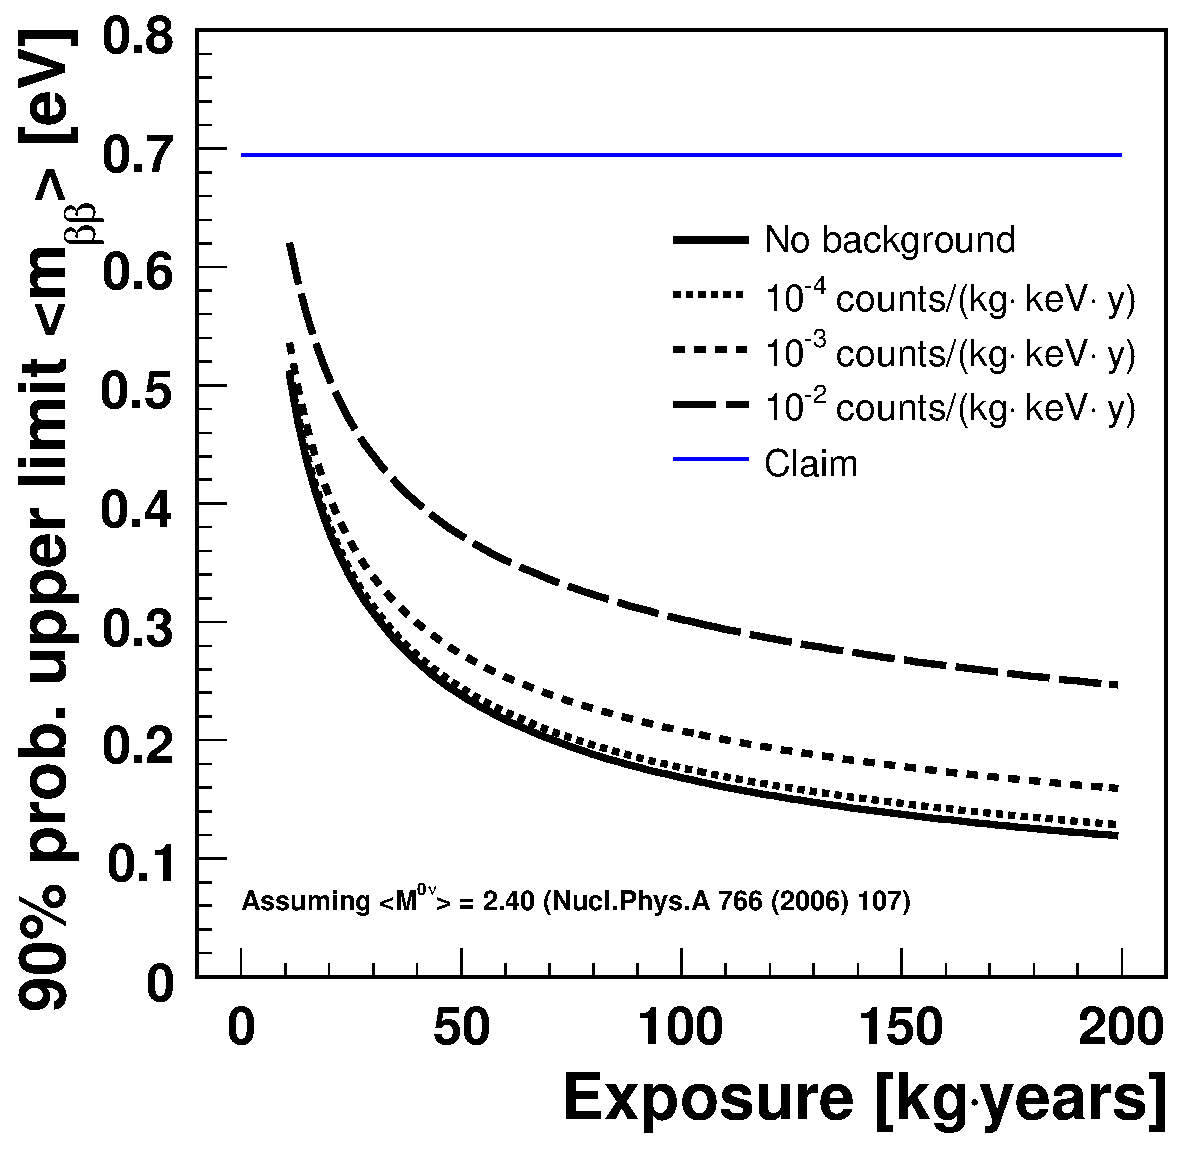
\includegraphics[width=0.45\textwidth]{limit_mass}  \hfil
  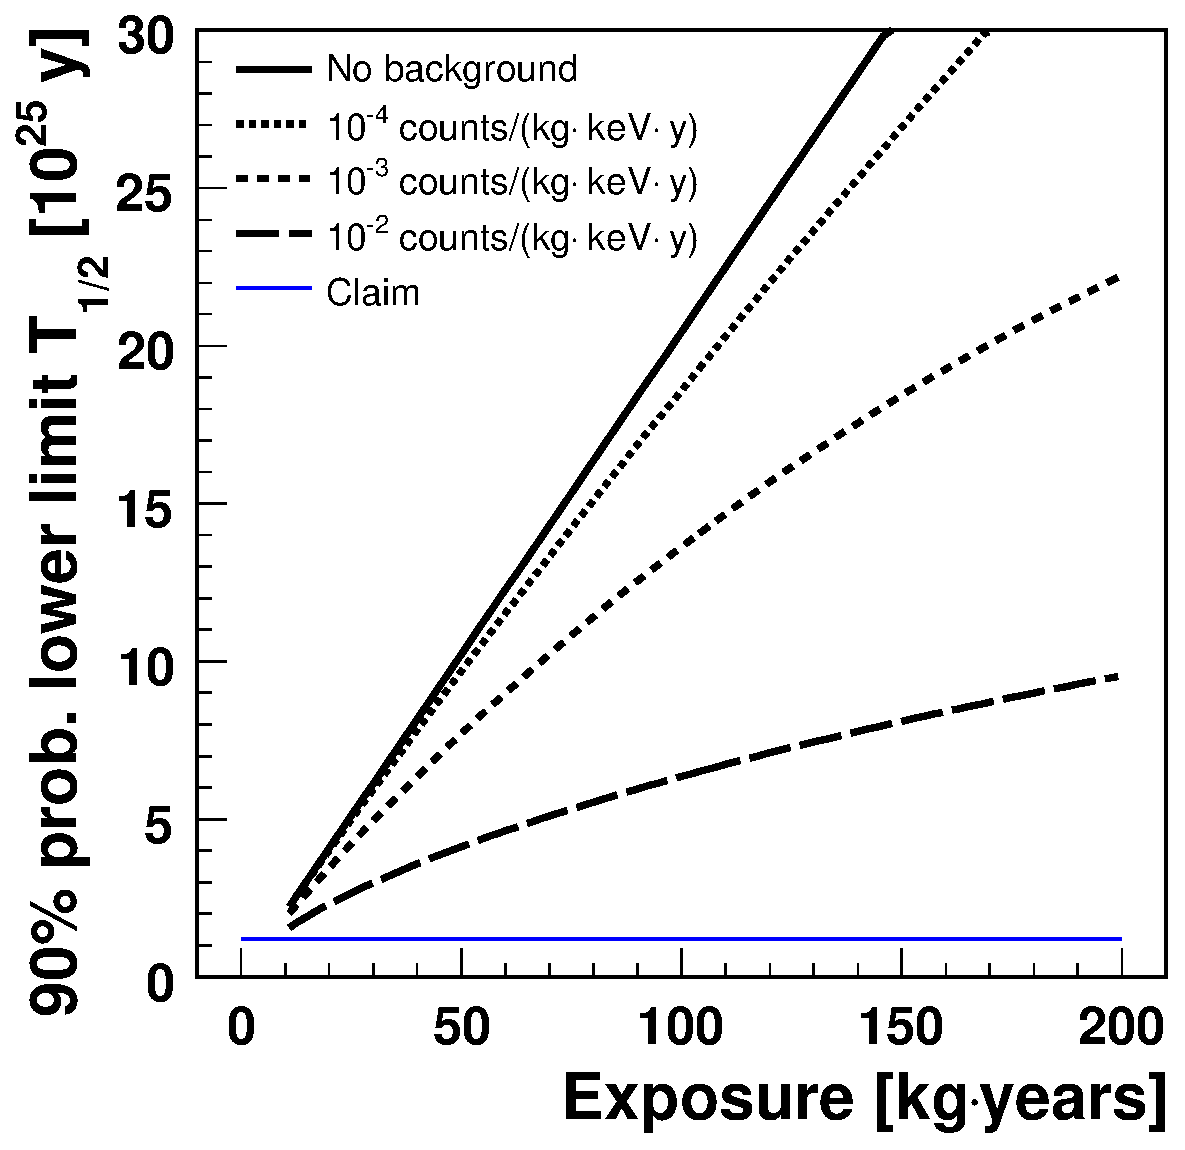
\includegraphics[width=0.45\textwidth]{limit_halflife}
  \caption{The expected 90\% probability lower limit on the half     lifetime for $0\nu\beta\beta$ decay (left) and the expected 90\%     probability upper limit on the effective Majorana neutrino mass     (right) versus the exposure under different background conditions.     Also shown is the half lifetime and the effective Majorana     neutrino mass for the claimed observation by H. V.     Klapdor-Kleingrothaus \textit{et al.}~\cite{Hei04}. All mass     values are determined from the half lifetime using the matrix     element reported in Ref~\cite{Rod07}.}
  \label{fig:gerda:limit}
\end{figure}

\subsection{General consideration}
\label{sec:gerda:gencon}
According to eq.~\ref{eq:gerda:mbb}, to design a $0\nu\beta\beta$ decay experiment with high sensitivity, \textit{i.e.} the capability to set a lower limit on $m_{\beta\beta}$, the following requirement needs to be fulfilled as much as possible:
\begin{itemize}
\item the source material $M$ should be as much as possible;
\item the natural abundance of the isotope under study should be large, or it is easy to enrich the isotope;
\item the calculation of the nuclear matrix element $|\mathcal{M}_{0\nu}|$ for this isotope should be accurate;
\item since $G_{0\nu}(Q,Z) \propto Q^{5}$, the $Q$-value should be large, and better to be larger than 2.6~MeV, in order to be above all the natural radioactive decay lines;
\item the signal detecting efficiency should be large;
\item the energy resolution should be good in order to have a small $\Delta E$;
\item last but not the least, the background level $b$ should be as low as possible.
\end{itemize}
After all, one needs to wait until a better upper limit on $T^{0\nu}_{1/2}$ could be set or an observation could be claimed.

Except for background suppression techniques, the experimental approach would be mostly determined by the choice of the source material. Table~\ref{tab:gerda:iso} presents a selection of isotopes used or planned to be used to search $0\nu\beta\beta$ decay. Also listed are their $Q$-values, nuclear matrix elements~\cite{Mut90, Rod07, Sim08, Cau08}, natural abundance $\kappa$ and properties important for the experimental design. Different experimental approaches can be classified into two categories: 1. the source material can be used to produce the detector; 2. the source is not the detector, the decay products need to be detected using equipment around the source.
\begin{table}[htbp]
  \centering
  \caption{A selection of possible source candidates for         $0\nu\beta\beta$ decay experiments. Also listed are their $Q$-values,     nuclear matrix elements, natural abundance $\kappa$ and properties     important for the experimental design.}
  \label{tab:gerda:iso}
  \begin{minipage}{\linewidth}
    \begin{tabular}{ccccc} \hline Isotope & $Q$ [MeV] &       $\mathcal{M}_{0\nu}$ & $\kappa$ [\%] & Properties \\\hline       $^{48}$Ca & 4.271 & 0.67\footnote{The values are from the ISM         (Interacting Shell Model) calculation~\cite{Cau08}.  The other         $\mathcal{M}_{0\nu}$ values with errors are from the QRPA         (Quasi-particle Random Phase Approximation)         calculations~\cite{Rod07}. The errors are from the measurement         of $2\nu\beta\beta$ experiments.} & 0.19 & CaF$_{2}$ \&       CaWO$_{4}$ is scintillator \\
      $^{76}$Ge & 2.039 & $4.51 \pm 0.17$ & 7.8 & semiconductor \\
      $^{82}$Se & 2.995 & $4.02 \pm 0.15$ & 9.2 & - \\
      $^{96}$Zr & 3.350 & $1.12 \pm 0.03$ & 2.8 & - \\
      $^{100}$Mo & 3.034 & $3.34 \pm 0.19$ & 9.6 & - \\
      $^{116}$Cd & 2.809 & $2.74 \pm 0.19$ & 7.5 &       CdZnTe\footnote{There are more than one isotope in the CdZnTe         crystal that could undergo $0\nu\beta\beta$ decay. The rest of         them are $^{70}$Zn with $Q = 1.001$~MeV, $\kappa = 0.62\%$,         $^{114}$Cd with $Q = 0.534$~MeV, $\kappa = 28.7\%$, $^{128}$Te         with $Q = 0.868$~MeV, $\kappa = 31.7\%$ and $^{130}$Te.} is       semiconductor; CdWO$_{4}$ is scintillator\\
      $^{124}$Sn & 2.287 & $2.11^{a}$ & 5.8 & semiconductor \\
      $^{130}$Te & 2.530 & $3.26 \pm 0.12$ & 35 & TeO$_{2}$ can be       used as bolometer\\
      $^{136}$Xe & 2.480 & $2.11 \pm 0.11$ & 8.9 & filling material of       time projection chamber\\
      $^{150}$Nd & 3.367 & $4.74 \pm 0.20$ & 5.6 & could be dissolved       in liquid scintillator\\
    \end{tabular}
  \end{minipage}
\end{table}

\subsection{Source is detector}
\label{sec:gerda:sed}
As shown in Table~\ref{tab:gerda:iso}, quit a few $0\nu\beta\beta$ decay candidates have special properties which allow them to be used as detectors at the same time. The advantages of this concept are 1. high energy resolution is easy to achieve; 2. large mass scale is possible. The disadvantages are 1. there are constraints on detector materials; 2. no event topology can be reconstructed.

$^{48}$Ca has the advantage of having the highest $Q$-value among all the candidates. Hence low background rate from natural radioactivities is expected. It also means a large phase space factor which enlarges $0\nu\beta\beta$ decay rate for a given Majorana mass. However, until now only few experiments have been carried out because of the low natural abundance of $^{48}$Ca. The most stringent limit on the $0\nu\beta\beta$ decay of $^{48}$Ca came from ELEGANT VI~\cite{Oga04} using CaF$_{2}$ scintillator. Two future experiments using CaF$_{2}$ and CaWO$_{4}$ as scintillator, respectively, are CANDLES~\cite{Ume06} and CARVEL~\cite{Zde05}. They aim at the sensitivity of $m_{\beta\beta} <$~(0.04-0.09)~eV.

The search for the $0\nu\beta\beta$ decay of $^{76}$Ge suffers from the natural radioactive decays due to the low $Q$-value of $^{76}$Ge. The enrichment of $^{76}$Ge of the source material is also needed in order to overcome the low natural abundance. However, semiconductor detectors made from high pure germanium crystals have been used as gamma spectrometers for years and have excellent energy resolution. The previous $^{76}$Ge $0\nu\beta\beta$ decay experiments include IGEX~\cite{Aal02} and Heidelberg-Moscow~\cite{Hei04}. GERDA~\cite{Sch05} is currently under construction and will be described in detail later. The planned future experiments include GERDA phase II, III and Majorana~\cite{Gai03, Aal04}. The GERDA and Majorana Collaborations have reached an agreement to share resources and knowledge where appropriate in their parallel development of the two different detector designs. The ultimate goal is to combine the strength of the two Collaborations in a future experiment that will employ the best technology for reaching a Majorana neutrino mass sensitivity of below 0.05~eV.

The Cobra experiment~\cite{Zub01, Ell02, Kie03} using a large array of CdZnTe semiconductors partially overcomes the disadvantages of the ``source = detector'' concept. The CdZnTe crystal contains up to 5 isotopes which could undergo $0\nu\beta\beta$ decay. Pixellated CdZnTe detector could also be operated as solid-state TPC and hence offer tracking capability which allows the event topology reconstruction. Another advantage of the CdZnTe detector is that it can be operated at room temperature. No large and complicated cooling facility is needed. However, the energy resolution of the CdZnTe detector currently is not as competitive as the germanium detector and TeO$_{2}$ bolometer.

The tungstate CdWO$_{4}$ is similar to CaWO$_{4}$, and can be used as scintillator. A comprehensive comparison between them can be found in page 27 of Ref.~\cite{Avi05}. The CdWO$_{4}$ crystal has less contamination and better background/signal discrimination power than the CaWO$_{4}$ crystal. The previous $0\nu\beta\beta$ decay experiments using CdWO$_{4}$ scintillators include the one performed by the Kiev-Florence collaboration in the Solotvina Underground Laboratory since 1989~\cite{Dan00, Dan03} and CAMEO~\cite{Bel00, Bel01}. The CAMEO project also proposes to exploit 1 ton of $^{116}$CdWO$_{4}$ detectors placed in one of the large underground neutrino detectors such as BOREXINO~\cite{Arp08}, SNO or KamLAND. The sensitivity is estimated as $m_{\beta\beta} < 0.02$~eV.

CUORICINO~\cite{Pre04}, the pilot experiment for the next generation $0\nu\beta\beta$ decay experiment CUORE~\cite{Arn04, Ard05}, just released a new upper limit of $m_{\beta\beta} <$~0.19-0.68~eV~\cite{Arn08} using TeO$_{2}$ bolometers. The TeO$_{2}$ bolometer has almost the same energy resolution as the germanium detector. $^{130}$Te has the highest natural abundance among all the $0\nu\beta\beta$ decay candidates. One could also dope other $0\nu\beta\beta$ decay isotopes into the bolometer, or some materials to make the TeO$_{2}$ crystal also a scintillator. The scintillating bolometer could provide more parameters helping background rejection, especially for surface contamination.

Xenon has the advantage of being used as the filling material of TPC (Time Projection Chamber). This would allow the reconstruction of the tracks of electrons from the beta decay, and hence leads to easy distinguishment of the $0\nu\beta\beta$ decay signal from the background. An experiment was carried out in the Gotthard underground laboratory using TPC filled with xenon gas enriched to 62.5~\% in $^{136}$Xe at a pressure of 5 bar~\cite{Lue98}. Currently, there are two experiments named EXO~\cite{Aki05} and XMASS~\cite{Kim05} proposing to use TPC filled with liquid xenon which can be used as scintillator at the same time.

$^{150}$Nd has the second highest $Q$-value, the biggest nuclear matrix element $\mathcal{M}_{0\nu}$ (though the uncertainty of $\mathcal{M}_{0\nu}$ is big) and relatively good natural abundance (enrichment is possible). These advantages make $^{150}$Nd a very suitable candidates for $0\nu\beta\beta$ decay search. In a follow up experiment of SNO, called SNO+~\cite{Zub07}, the old SNO infrastructure will be filled with Nd-loaded liquid scintillator instead of D$_{2}$O. Although the energy resolution of the detector will not be as good as that of other existing experiments, the amount of isotope that could be suspended in the scintillator is very large (0.1\% load of natural Nd corresponds to 56~kg of $^{150}$Nd). Based on preliminary simulations, loading with enriched Nd at 0.1\% level SNO+ would have the sensitivity of $m_{\beta\beta}$ down to 0.03~eV.

\subsection{Source is not  detector}
\label{sec:gerda:sued}
The advantages of using external detector are 1. the source material could be changed so that several $0\nu\beta\beta$ decay candidates could be measured in the same experiment; 2. using tracking devices the event topology could be reconstructed which leads to excellent background/signal distinguishment. The disadvantages are 1. normally the energy resolution is not good; 2. in order to release the beta decay electrons, the source has to be made into thin foil and hence large mass scale experiment is difficult to realize.

The previous experiments include TGV I and II~\cite{Ste98, Ste00,   Ste06}, NEMO I~\cite{Das91}, II~\cite{Arn95} and III~\cite{Arn05,   Arn07}. In TGV Cd plates were put in between germanium spectrometers. In NEMO the source foils (Ca, Se, Zr, Cd, Mo, Te and Nd) were fixed between two tracking volumes composed of many drift cells. The planned future experiments include SuperNEMO~\cite{Sne08}, MOON~\cite{Nak06} and DCBA~\cite{Ish05}. Based on the NEMO III experience, SuperNEMO aims at the sensitivity of $m_{\beta\beta} \sim 0.03$~eV. In MOON, enriched $^{100}$Mo foils will be interleaved with plastic scintillators which work as a calorimeter as well as an active shield. The designed sensitivity of MOON is $m_{\beta\beta} \sim 0.03$~eV. DCBA consists of tracking chambers, a solenoid magnet and veto-counters for cosmic rays. Thin source plates will be installed in tracking detectors located in a uniform magnetic field. The designed sensitivity is $m_{\beta\beta} \sim 0.05$~eV.


\section{The GERDA experiment}
\label{sec:gerda:concept}

\subsection{Concept}
\label{sec:gerda:concept}

\subsection{Status}
\label{sec:gerda:status}


%%% Local Variables:
%%% mode:latex
%%% TeX-master: "thesis"
%%% End:
